% "{'classe':('PSI'),'chapitre':'slci_correcteurs','type':('colle'),'titre':'Réglage d\\'un correcteur P et d\\'un correcteur à avance de phase', 'source':'Pôle Chateaubriand -- Joliot Curie','comp':('C1-02','C2-04'),'corrige':False}"
%\setchapterimage{bandeau}
\chapter*{Colle \arabic{cptColle} \\ 
Réglage d'un correcteur P et d'un correcteur à avance de phase -- 
\ifprof Corrigé \else Sujet \fi}
\addcontentsline{toc}{section}{Colle \arabic{cptColle} :
Réglage d'un correcteur P et d'un correcteur à avance de phase -- 
\ifprof Corrigé \else Sujet \fi}

\iflivret \stepcounter{cptColle} \else
\ifprof  \stepcounter{cptColle} \else \fi
\fi

\setcounter{question}{0}
\marginnote{Pôle Chateaubriand -- Joliot Curie.}
\marginnote[1cm]{
\UPSTIcompetence[2]{C1-02}
\UPSTIcompetence[2]{C2-04}}

%\begin{marginfigure} [4cm]
%\includegraphics[width=\linewidth]{fig_01a}
%\end{marginfigure}



\subsection*{Correction proportionnelle}
Soit $F(p)$ la FTBO d'un système bouclé à retour unitaire. Les diagrammes de BODE de $F(p)$ sont représentés
sur la figure ci-dessous.

\question{Déterminer les marges de phase et de gain du système, puis conclure quant à sa stabilité.}


On décide d’ajouter au système un correcteur série de type proportionnel. On note $K_p$ le gain de ce
correcteur.

\question{Déterminer la valeur de $K_p$ permettant d’obtenir une marge de gain $M_G =\SI{12}{dB}$.}

\question{Déterminer la nouvelle marge de phase du système.}

\question{En le justifiant, déterminer l’erreur de position du système corrigé pour une consigne indicielle.}


\subsection*{Correction intégrale -- Asservissement en accélération}
%\setcounter{exo}{0}
\begin{marginfigure}
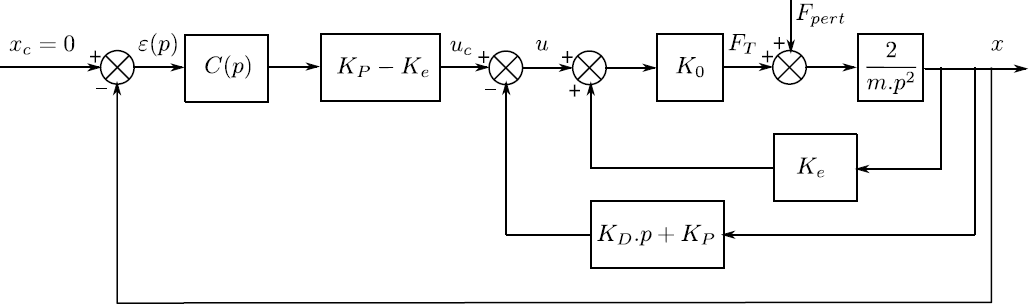
\includegraphics[width=\linewidth]{fig_02}
\end{marginfigure}

On désire contrôler l'accélération $\gamma(t)$ d'un plateau. Pour cela, un capteur d'accélération, fixé sur le plateau
et de sensibilité $B$, est utilisé dans la chaîne de retour du système. Le moteur permettant la motorisation du
plateau est modélisé par la fonction de transfert : $H(s)=\dfrac{A}{1+\tau s}$. 
On modélise le correcteur par la fonction de transfert $C(s)$.

On a $A=\SI{100}{g.m.s^{-2}.V^{-1}}$, $\tau=\SI{0,2}{s}$ et $B=10^{-2}\,\text{g}^{-1}\text{V}\text{m}^{-1}\text{s}^{-2}$.

\question{Quelle doit être la fonction de transfert du transducteur $T(s)$ qui traduira l’accélération de consigne $\Gamma_c(s)$ en tension $E(s)$.}

On applique à l’entrée du système une consigne d’accélération $\gamma_c=20 g$.

Système asservi sans correction : $C(s)=1$.
\question{Déterminer l'expression de la fonction de transfert en boucle fermée de ce système. Identifier les différents paramètres de cette fonction. Réaliser l'application numérique.}

\question{Calculer le temps de réponse à 5\% de ce système pour une entrée en échelon.}

\question{Donner la valeur de l'accélération en régime permanent. Ce système est-il précis ? Donner l'erreur en régime permanent.}

\question{Donner l'allure de la réponse de ce système en précisant les points caractéristiques.}

\subsection*{Système asservi avec correction intégrale : $C(s)=\dfrac{1}{s}$.}

%\begin{marginfigure}
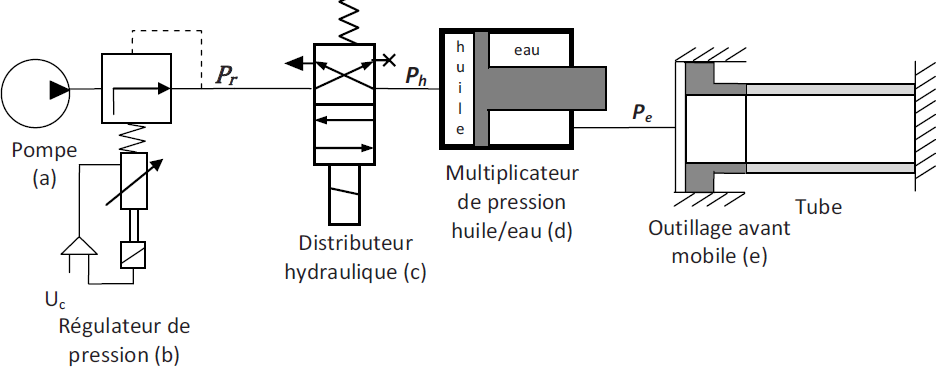
\includegraphics[width=\linewidth]{fig_01}
%\end{marginfigure}


\question{Déterminer l'expression de la fonction de transfert en boucle fermée de ce système. Identifier les
différents paramètres de cette fonction. Réaliser l'application numérique.}

\question{Calculer le temps de réponse à 5\% de ce système pour une entrée en échelon.}

\question{Donner la valeur de l'accélération en régime permanent. Ce système est-il précis ? Donner l'erreur en
régime permanent. Pouvait-on prévoir ce résultat.}

\question{Conclure en comparant le comportement du système avec et sans correction.}


\ifprof
\else
\begin{marginfigure}[-3cm]
\centering

\includegraphics[width=3cm]{Cy_03_01_Colle_04_P_I_qr}
\end{marginfigure}
\fi

\ifprof
\begin{center}
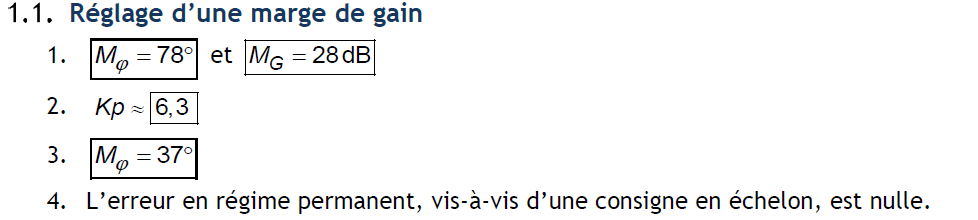
\includegraphics[width=\linewidth]{cor_01}
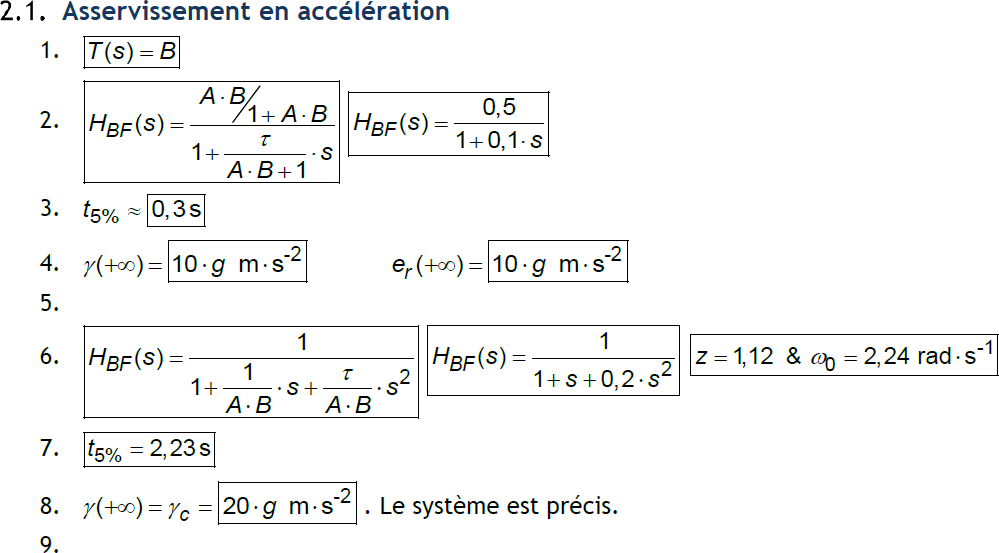
\includegraphics[width=\linewidth]{cor_02}
\end{center}
\else
\fi
